\chapter{Háttérismeretek}

\section{Kapocsolódó munkák}
%TODO: 

\section{SysML}

A SysML egy általános célú modellezési nyelv, melyet elsősorban rendszermérnökök használnak. A nyelvvel komplex rendszereket tudunk leírni akár magasabb szintű logikai felépítés és viselkedés vagy nagyon alacsony absztrakciókon fizikai felépítést, viselkedést. A különböző absztrakciós szinteken létrehozott modelleket egymáshoz tudjuk rendelni, például egy logikai funkciót milyen fizikai egységek látnak el.

A SysML-t mint ahogyan az UML-t is az OMG fejlesztette annak leszűkítésével majd speciális elemek bevezetésével. Ezzel egy még az UML-nél is általánosabb fogalomrendszert hoztak létre.
Az adott nyelv által definiált elemeket és azok kapcsolatát metamodell írja le. Az UML metamodellje és ennek ismerete éppen ezért jelentős szerepet töltött be a fejlesztés során, főleg hogy a SysML-nek nincs a hagyományos értelemben vett külön metamodellje, hanem UML profilok segítségével van a nyelv definiálva. 

%TODO kifejteni

%TODO szep kep 

A modellek amikkel a továbbiakban foglalkozok logikai struktúrákat és viselkedést írnak le. A viselkedés modellek főként állapotgépekre szűkülnek melyeket állapottérképek (Statechart Diagram) segítségével tudunk ábrázolni. A rendszer logikai felépítését vagy funkcionális architektúráját (Functional Architecture) pedig Internal Block Diagram (IBD) segítségével.



%TODO IBD

\section{MagicDraw}

A MagicDraw egy modellező eszköz mellyel UML modelleket tudunk készíteni. Ahhoz, hogy SyML-ben is tudjunk modelleket készíteni egy beépülő modulra van szükségünk (kivéve ha Cameo System Modellert használunk ami a SysML pluginnal integrálva szállít). A MagicDraw az iparban egy egyre inkább elterjedt eszköz. Szigorúan követi az UML és SysML szabványt.


%TODO felulet stb...


\section{Felhasznált technológiák}
\subsection{Eclipse Modeling Framework}
\section{Modelltranszformációk}

Az ipari standardok mellett sok speciális modellezési nyelv is létezik, amelyek megannyi céllal és eszközkészlettel jöttek létre. Ezek között vannak magas absztrakciójú általánosabb nyelvek és alacsony szintűek is amik egy része olyan formalizmusokra épül amik felett bizonyos problémákra matematikai eszközökkel tudunk megoldást keresni.

A modellvezéreltség egyik alapötlete, hogy különböző modellekből származtatni tudunk más modelleket feltéve, hogy elegendő információ áll rendelkezésünkre a konverzió elvégzéséhez. Ezt a fajta származtatási folyamatot modelltranszformációnak nevezzük. A modelltranszformációk használata lehetővé teszi, hogy ne csak azokat a technológiákat használjuk modellünk feldolgozására melyek speciálisan az adott modellezési nyelvhez készültek hanem a modelleket megpróbáljuk átalakítani - lehetőleg a szemantikai tartalom megőrzésével és automatizáltan - egy olyan modellezési nyelvre amelyhez már létezik az általunk használni kívánt funkcionalitást támogató technológia.

Fontos megjegyezni, hogy előfordulhatnak olyan esetek is amikor a modell transzformáció komplexitása és elkészítésének költsége, ha egyáltalán lehetséges ilyet készíteni, nagyobb mintha speciálisan az adott nyelvhez készítenénk egy speciális eszközt ami megvalósítja az állvárt funkcionalitást.

\subsection{VIATRA}

A VIATRA egy keretrendszer mely lehetővé teszi eseményvezért modell transzformációk fejlesztését. Ehhez egy inkrementális modell lekérdezéseket leíró nyelvre a VIATRA Query Language-re támaszkodik. A létrehozott transzformációkat egy reaktív Query Engine futtatja és tartja karban.

A VIATRA használata jelentősen megkönnyíti a modellekkel való munkát, bár én elsősorban a modell lekérdezés részére támaszkodtam a dolgozat elkészítése alatt.

\section{MagicDraw állapottérkép verifikációs plugin}

\subsection{MagicDraw - Gamma transzformáció}

A MagicDraw beépülő modul fő célja SysML állapottérképek formális verifikációja, ehhez vagy megpróbálunk írni egy eszközt amely képes közvetlen ilyen állapottérképeken dolgozni vagy átalakítani egy olyan modellezési nyelvre amelyhez rendelkezik olyan eszköz ami ezt el tudja végezni. Ilyen lehetett volna például az \uppaal, ez viszont jóval alacsonyabb szintű mint a modellek amiket ellenőrizni szerettem volna ezért a transzformáció elvégzése potenciálisan nagyon komplex lett volna. Ilyen transzformációt azonban már készítettek egy állapottérkép modellező nyelv a Gamma és az \uppaal  között, ezért ahelyett, hogy közvetlen \uppaal modelleket készítenél Gamma modelleket transzformálok. Ezzel nem csak az \uppaal-ra való transzformálhatóságot és a formális verifikációt nyerem, hanem mindenm olyan funkciót ami a Gammához készül és a transzformációhoz szükséges megfeleltetések is egyszerűsödnek valamelyest.

\subsection{Verifikáció menete}

A verifikáció elvégzése a MagicDraw beépülő modul szemszögéből négy lépésből áll : 
\begin{itemize}
	\item MagicDraw modellek Gammává transzformálása
	\item Gamma modellek \uppaal modellé transzformálása (ezt a Gamma keretrendszer végzi el)
	\item tulajdonságok ellenőrzése UPPAAL segítségével
	\item Eredmény megjelenítése
\end{itemize}
Ezt a folyamatot \refstruc{fig:preliminaries-verif} szemlélteti. A Gamma által elvégzett lépéseket a zöld "Gammák" jelölik a modellben. Az ábrán a verifikációt a "Módosított Query Generátor" kezdeményezi, mely szintén a "Gamma" jelölést kapta. Ennek oka, hogy a beépülő modul ezen verziójában az ellenőrizendő tulajdonságok megadása még nem volt kiforrott ezért egy a Gamma keretrendszerből átemelt megoldás segítségével lehetett ezeket megadni és a verifikációt kezdeményezni. Jelen dolgozatban a továbbiakban szó lesz többek között ennek a kiváltásáról egy előnyösebb ebben a környezetben felhasználóbarátabb megoldással.

\begin{figure}[!ht]
	\centering
	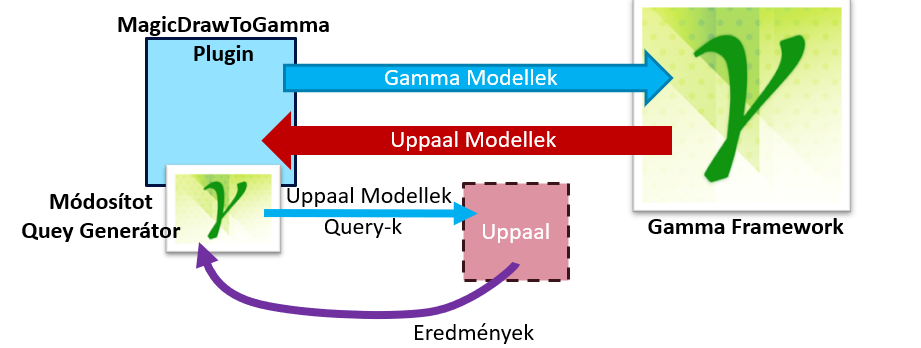
\includegraphics[width=150mm, keepaspectratio]{figures/preliminaries/concept.png}
	\caption{Verifikáció menete a pluginban}
	\label{fig:preliminaries-verif}
\end{figure}
